\section{Udvælgelse af gestik-par til at skrue op og ned for musikken}
\label{TestresultaterVolumen}
%
Udvælgelsen af hvilket gestik-par, der skal knyttes til at skrue op og ned for musikken foretages på baggrund af testpersonernes udsagn. I \fullref{app:TestresultaterVolumenDaarlig} analyseres testpersonernes respons i forhold til hvilke gestik-par de mindst kan lide og på baggrund af den analyse ekskluderes gestik-par 6, gestik-par 7 og gestik-par 8 fra yderligere undersøgelser. Dette medfører at udvælgelsen af hvilket gestik-par, der skal knyttes til at skrue op og ned kun foretages på gestik-par 1, gestik-par 2, gestik-par 3, gestik-par 4, gestik-par 5 og gestik-par 9.\blankline
%  
I nedenstående \autoref{tab:GestikParITopTreVolumen} fremgår samtlige testpersoners top tre rangering, hvor der ikke er taget forbehold for hvorvidt testpersonerne har inkluderet et gestik-par, som der på baggrund af \fullref{app:TestresultaterPauseDaarlig} er blevet ekskluderet.
%
\begin{table}[H]
	\centering
	\begin{tabular}{ | p{3cm} | p{3cm} | p{3cm} | p{3cm} |}
		\hline
		& 1. Plads & 2. Plads & 3. Plads \\ \hline
		Testperson 1 & Gestik-par 2 & Gestik-par 6 & Gestik-par 3 \\ \hline
		Testperson 2 & Gestik-par 4 & Gestik-par 5 & Gestik-par 6 \\ \hline
		Testperson 3 & Gestik-par 9 & Gestik-par 4 & Gestik-par 2 \\ \hline
		Testperson 4 & Gestik-par 3 & Gestik-par 1 & Gestik-par 2 \\ \hline
		Testperson 5 & Gestik-par 6 & Gestik-par 1 & Gestik-par 5 \\ \hline
		Testperson 6 & Gestik-par 3 & Gestik-par 4 & Gestik-par 8 \\ \hline 
		Testperson 7 & Gestik-par 2 & Gestik-par 5 & Gestik-par 3 \\ \hline
		Testperson 8 & Gestik-par 1 & Gestik-par 4 & Gestik-par 3 \\ \hline
		Testperson 9 & Gestik-par 9 & Gestik-par 1 & Gestik-par 4 \\ \hline
		Testperson 10 & Gestik-par 3 & Gestik-par 5 & Gestik-par 2 \\ \hline
		Testperson 11 & Gestik-par 3 & Gestik-par 4 & Gestik-par 8 \\ \hline
		Testperson 12 & Gestik-par 4 & Gestik-par 3 & Gestik-par 5 \\ \hline
		Testperson 13 & Gestik-par 3 & Gestik-par 2 & Gestik-par 1 \\ \hline
		Testperson 14 & Gestik-par 2 & Gestik-par 6 & Gestik-par 5 \\ \hline
		Testperson 15 & Gestik-par 3 & Gestik-par 4 & Gestik-par 9 \\ \hline
		Testperson 16 & Gestik-par 1 & Gestik-par 3 & Gestik-par 9 \\ \hline
		Testperson 17 & Gestik-par 2 & Gestik-par 9 & Gestik-par 3 \\ \hline
		Testperson 18 & Gestik-par 4 & Gestik-par 2 & Gestik-par 9 \\ \hline
	\end{tabular}
	\caption{Oversigt over samtlige testpersoners top tre i forbindelse med at skrue op og ned for musikken.}
	\label{tab:GestikParITopTreVolumen}
\end{table}
\noindent
%
Få at få et overblik over hvor ofte de ni forskellige gestik-par individuelt indgår på enten en første, anden eller tredje plads i top tre rangeringen opstilles følgende \autoref{fig:SamletTopTreVolumen}, som bygger på data fra \autoref{tab:GestikParITopTreVolumen}. 
%
\begin{figure}[H]
	\centering
	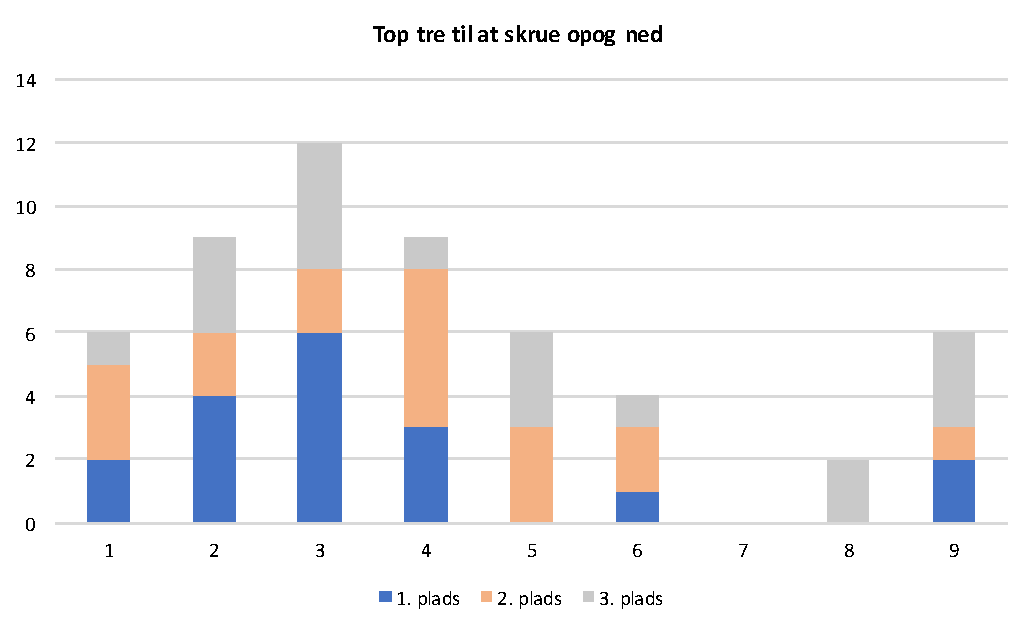
\includegraphics[resolution=300,width=0.9\textwidth]{Test1/DatabehandlingGrafer/TopTreVolumen}
	\caption{Barplot over hvordan hvert gestik-par indgår i testpersonernes top tre i forhold til at skrue op og ned.}
	\label{fig:SamletTopTreVolumen}
\end{figure}
\noindent
%
Da der er tre gestik-par, som er blevet ekskluderet, kan ovenstående  \autoref{tab:GestikParITopTreVolumen} med fordel opsummeres både i forhold til at fjerne de tre gestik-par men også i forhold til at opsummere hvor mange gange de seks tilbageværende gestik-par indgår i top tre rangeringen. 
%
\begin{table}[H]
	\centering
	\begin{tabular}{ | p{2.4cm} | p{2.4cm} | p{2.4cm} | p{2.4cm} |p{2.4cm}|}
		\hline
		& 1. Plads & 2. Plads & 3. Plads & I alt \\ \hline
		Gestik-par 1 & 2 & 3 & 1 & 6\\ \hline
		Gestik-par 2 & 4 & 2 & 3 & 9\\ \hline
		Gestik-par 3 & 6 & 2 & 4 & 12\\ \hline
		Gestik-par 4 & 3 & 5 & 1 & 9\\ \hline 
		Gestik-par 5 & 0 & 3 & 3 & 6\\ \hline
		Gestik-par 9 & 2 & 1 & 3 & 6\\ \hline
	\end{tabular}
	\caption{Oversigt over dels hvor mange gange hvert gestik-par indgår i samtlige testpersoners top tre i forbindelse med at skrue op og ned for musikken og dels over hvor mange gange et gestik-par sammenlagt indgår i en top tre.}
	\label{tab:GestikParITopTreVolumenOversigt}
\end{table}
\noindent
%
De to testpersoner, som begge har tildelt gestik-par 1 en første plads forbinder bevægelsen med noget de er vant til; at dreje på en knap for at skrue op. Gestik-par 1 illustreres på \autoref{fig:GestikPar1Volumen}. Derudover påpeger testperson, 8 at i forhold til bevægelsen i gestik-par 2 så er gestik-par 1 tydeligere og at gestik-par 1 er naturlig. Gestik-par 2 illustreres på \autoref{fig:GestikPar2Volumen}. I tillæg påpeger testperson 16, at bevægelsen i gestik-par 1 så mere behagelig ud sammenlignet med gestik-par 2, som testpersonen fandt ukomfortabel. En af årsagerne til at testperson 16 vurderer at gestik-par 2 er ukomfortabel skyldes formentlig, at i videooptagelsen bliver gestik-par 2 ikke gengivet lige så afslappet, som det var hensigten. I videooptagelsen fremgår det at nærmest hele armen skal i bevægelse; fra skulderen og ud til fingrene, hvilket ikke er hensigten med gestikken. Hensigten med gestik-par 2 er, at bevægelsen bør dannes ud fra en kombination mellem underarmen, håndleddet og fingrene, så det tilnærmelsesvist er den samme bevægelse, som går igen ved gestik-par 1. Sammenholdes testperson 16’s udsagn med testpersonens bevægelser, når testpersonen opfordres til at komme med et forbedringsforslag, så begynder testpersonen rent faktisk med at gengive bevægelsen i gestik-par 2 og det er først når testlederen konfronterer testperson 16, at testpersonen gengiver gestik-par 1. Når testperson 16 afslutningsvist bliver bedt om, at gengive sine foretrukne gestikker, så er det heller ikke gestik-par 1 testpersonen gengiver men starten på gestik-par 2, illustreret på \autoref{fig:GestikPar2Volumen}, og når der så skrues op eller ned gøres det med en flad og udstrakt hånd i en cirkulærbevægelse. Sammenholdes det testpersonen giver udtryk for, med hvad testpersonen rent faktisk gør, så stemmer det ikke overens i forhold til gestik-par 1, som illustreres på \autoref{fig:GestikPar1Volumen}. Det tyder derfor på, at testpersonen formentligt foretrækker noget, der tilnærmelsesvist minder om gestik-par 2, men særligt foretrækker en cirkulærbevægelse.
%
\begin{figure}[H]
	\centering
	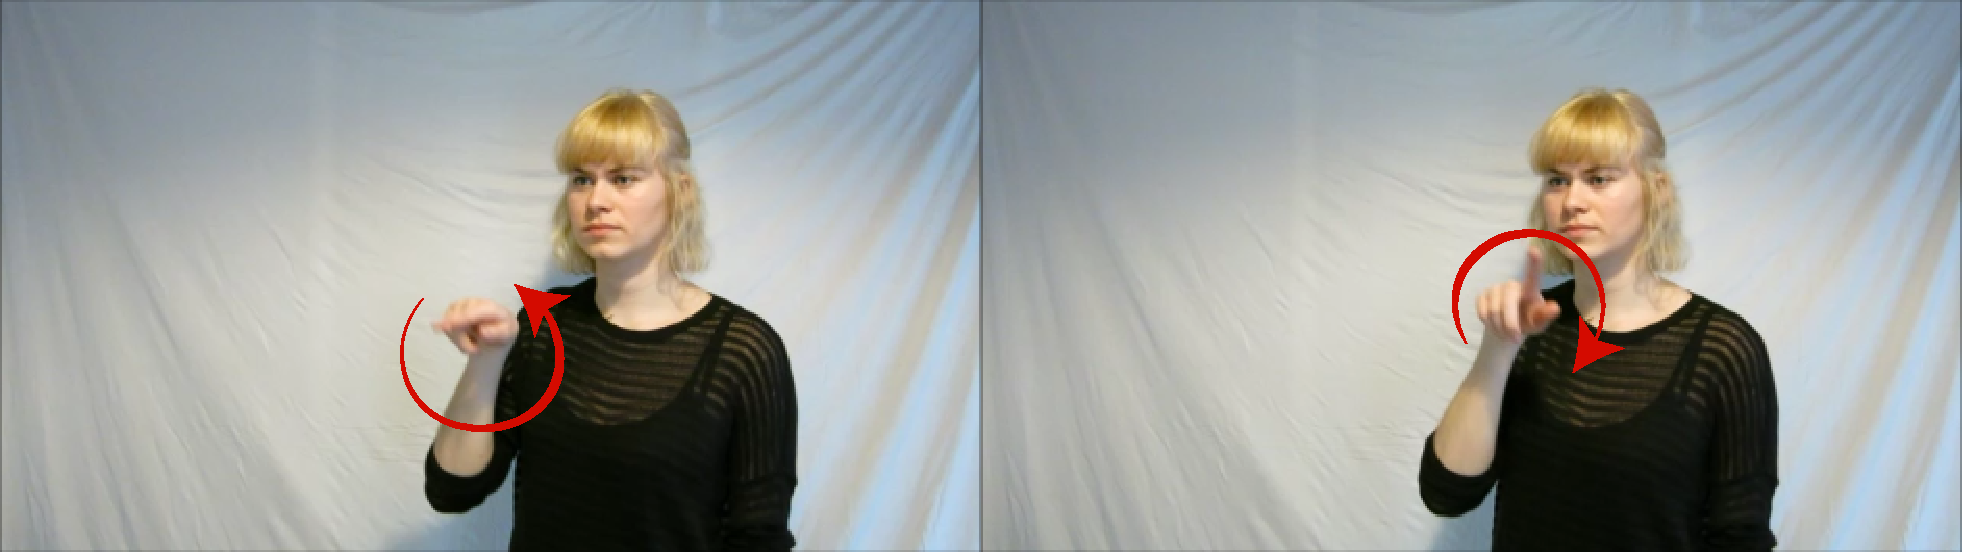
\includegraphics[resolution=300,width=0.9\textwidth]{Test1/Gestik-par/Gestik1_Volumen}
	\caption{Illustration af gestik-par 1; cirkulærbevægelse med pegefingeren i urets retning for at skrue op og mod uret for at skrue ned.}
	\label{fig:GestikPar1Volumen}
\end{figure}
\noindent
%
Baseret på testperson 4’s udsagn, så tyder det ikke på, at der er en særlig årsag til at gestik-par 1 er rangeret højere end gestik-par 2. Testpersonen giver udtryk for, at det er en naturlig bevægelse og at det er det testpersonen tænker, når der skal skrues op eller ned for noget. Testperson 5 giver udtryk for, at gestik-par 1 er intuitiv, nem at forstå, det er universelt så alle kan gengive bevægelsen, bevægelsen kan laves overalt og i forskellige størrelser. Derudover pointerer testpersonen, at gestik-par 1 er hurtigere at gengive end gestik-par 2. Dog giver testperson 5 først udtryk for, at kunne lide, hvad testpersonen definerer som volumen-knappen, svarende til gestik-par 2, som illustreres på \autoref{fig:GestikPar2Volumen}. Årsagen til at gestik-par 2 ikke indgår i testpersonens top tre, er fordi testpersonen finder den langsom at gengive. Testperson 9 tildeler først gestik-par 1 en første plads, men efter at have prøvet det tildeler testpersonen gestik-par 9 første pladsen. Gestik-par 9 illustreres på \autoref{fig:GestikPar9Volumen}. Testpersonen giver udtryk for, at foretrække gestikker, som kun kræver én hånd og som ikke distraherer testpersonens barn. Derudover kommenterer testpersonen, at gestik- par 1 virkede forholdvis overskuelig og nem. Ifølge testperson 9 fravælges gestik-par 2 fordi bevægelsen var stor og klodset, hvilket indikerer at hensigten med gestik-parret igen er fejlfortolket.

Med udgangspunkt i testperson 13’s udsagn er det ikke entydigt hvorfor testpersonen har tildelt gestik-par 1 en trejde plads, men testpersonen giver udtryk for, at de cirkulærebevægelser er sjove og at det minder om en knap. Derudover foretrækker testpersonen ligeledes, at gestikkerne kun kræver én hånd.
%
\begin{figure}[H]
	\centering
	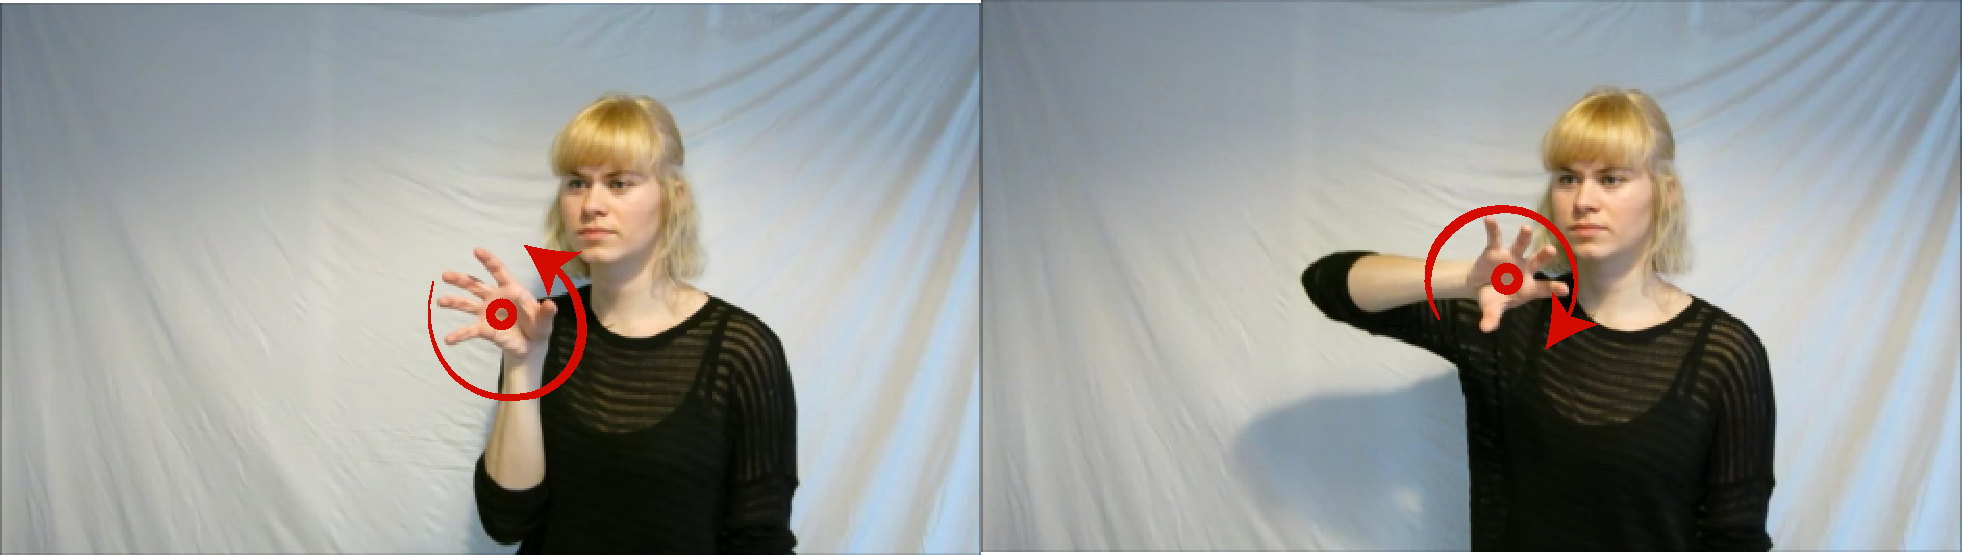
\includegraphics[resolution=300,width=0.9\textwidth]{Test1/Gestik-par/Gestik2_Volumen}
	\caption{Illustration af gestik-par 2; cirkulærbevægelse med halv bøjede fingrene, ligesom hvis det var en dreje-knap, der blev brugt. Der skal drejes med uret for at skrue op og mod uret for at skrue ned.}
	\label{fig:GestikPar2Volumen}
\end{figure}
\noindent
%
Seks ud af de ni testpersoner, som har inkluderet gestik-par 2 i sin top tre, forbinder gestikken med en drejeknap, som de i forvejen er vant til at interagere med for at skrue op eller ned på et anlæg, jævnfør \autoref{fig:GestikPar2Volumen}. Tre ud af de fire, som har tildelt gestik-par 2 en første plads, kommenterer, at de finder bevægelsen naturlig. Ifølge testperson 1, så tænkte testpersonen på gestik-par 2 allerede før testpersonen blev præsenteret for gestik-parret. Både testperson 17, testperson 18 og testperson 3 giver udtryk for, at bevægelsen giver mening for at skrue op eller ned for musikken. Igen vælger testperson 14 gestikker ud fra hvad der ikke naturligt forekommer, når testpersonen normalvist gestikulerer, hvorfor testpersonen har tildelt gestik-par 2 en første plads. Lignende argumenter fremsættes af testperson 18, som påpeger at bevægelsen i gestik-par 2 er så specifik, at det ikke er en bevægelse, der fejlagtigt opstår, jævnfør \autoref{fig:GestikPar2Volumen}. Derudover kommenterer testperson 18, at det er behageligt at dreje lyden op. Ligesom det er nævnt ved gestik-par 1, så giver testperson 13 udtryk for dels at cirkulærbevægelser er sjove og dels foretrækker en-hånds gestikker. Ifølge testperson 10, så er gestik-par 2 både intuitiv og nem at huske.

Udover at bevægelsesmængden i gestik-par 2 ikke behøver, at være så udtryksfuld, som det blev illustreret i videooptagelser, så er det kun testperson 14, som har et forbedringsforslag. Testperson 14 foreslår, at den ikke-dominante hånd, altså hånden, som ikke skal foretage cirkelbevægelsen, inkluderes, så det kræver begge hænder at skrue op og ned. I og med at størstedelen af testpersonerne foretrækker gestikker, som kun kræver én hånd, afvises foreslaget, men det tages til eftertrakning, at der måske skal være et nyt element i gestik-par 2. Et forslag til det er, at der først skal gives et form for tegn, hvorefter det er muligt at skrue op eller ned. Da flere testpersoner giver udtryk for, at de forbinder gestik- par 2 med en drejeknap, så kunne tegnet muligvis være en indikation af, at brugeren tager fat i selve knappen, før der enten drejes med eller mod uret.

En af fordelene ved at vælge gestik-par 2 fremfor gestik-par 1 er, at gestik-par 2 oftere indgår i testpersonernes samlede top tre, jævnfør \autoref{tab:GestikParITopTreVolumenOversigt}. Det anses ydermere for at være en fordel, at flere testpersoner forbinder bevægelsen i gestik-par 2 med noget de i forvejen er vant til, fordi de så ikke nødvendigvis behøver at lære noget nyt. Derudover antages det, at størstedelen af de personer, som har \textit{high-end} lydudstyr formentlig også har en forstærker, hvorpå lydstyrken normalvist ændres ved at dreje på en drejeknap, hvilket formentlig vil gøre det lettere for brugeren, at koble gestik-par 2 til den funktion. Ydermere påpeger både testperson 14 og testperson 18, at bevægelsen i gestik-par 2 ikke er en bevægelse, der normalvist indgår i ens naturlige gestikulation. Med forbehold for, at gestik-par 2 ikke nødvendigvis skal gengives på præcis samme måde, som det fremgår i videooptagelsen og på \autoref{fig:GestikPar2Volumen}og at der muligvis først skal være en indikation af, at nu skal der skrues op eller ned, så vurderes det, at gestik-par 2 egner sig bedre end gestik-par 1 til at skrue op og ned.
%
\begin{figure}[H]
	\centering
	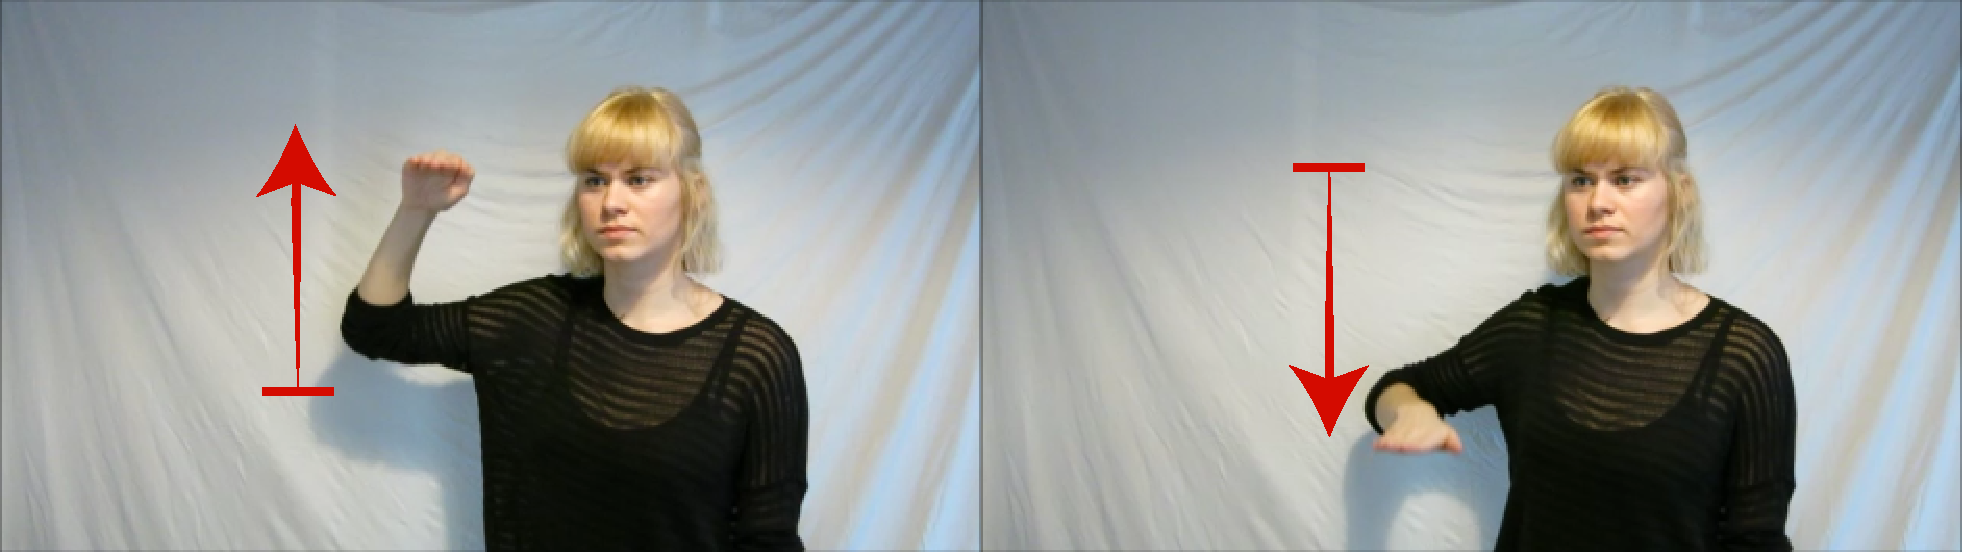
\includegraphics[resolution=300,width=0.9\textwidth]{Test1/Gestik-par/Gestik3_Volumen}
	\caption{Illustration af gestik-par 3; horisontal hånd løftes vertikalt med håndfladen nedad for at skrue op og for at skrue ned sænkes hånden vertikalt med håndfladen nedad.}
	\label{fig:GestikPar3Volumen}
\end{figure}
\noindent
%
På \autoref{fig:SamletTopTreVolumen} fremgår det, at gestik-par 3 er det gestik-par, som sammenlagt indgår flest gange i testpersonernes top tre; 12 gange i alt. På \autoref{fig:GestikPar3Volumen} illustreres gestik-par 3. Det tyder på, at ligesom ved de to foregående gestik-par, så foretrækker de testpersoner, som har tildelt gestik-par 3 en første plads, ligeledes at bevægelsen kan gøres med én hånd. Testperson 4 har tildelt gestik-par 3 en første plads ud fra, hvad der passede godt til det testpersonen valgte til pause og start, hvilket var gestik-par 1, jævnfør \autoref{fig:GestikPar1Volumen}. I og med at det gestik-par blev sorteret fra til pause og start, så er det ikke sikkert, at testpersonen stadig vil tildele gestik-par 3, til at skrue op og ned, en første plads. Testperson 10 giver, foruden at gestik-par 3 er intuitiv og nem at huske, udtryk for at bevægelsen passer godt til det den skal gøre. Lignende tendens går igen ved testperson 11; som foruden at vurdere gestik-par 3 som værende både logisk og intuitiv, giver udtryk for, at hvis der skal skrues op, så bør det være med en opadgåendebevægelse. Ifølge testperson 6 er gestik-par 3 naturlig og nemmere at udføre, i forhold til hvis der skal være en bestemt reference, som der blandt andet er i gestik-par 5, jævnfør \autoref{fig:GestikPar5Volumen}. Testperson 13 har svært ved uddybe hvorfor gestikkerne er rangeret i den rækkefølge, som fremgår af \autoref{tab:GestikParITopTreVolumen}, men testpersonen giver udtryk for godt, at kunne lide de gestik-par, hvor hånden enten skal hæves eller sænkes for at skrue op og ned. Både testperson 6 og testperson 13 giver udtryk for, at det er nemt at udføre bevægelserne i gestik-par 3. I tillæg kommenterer testperson 15, at gestik-par 3 er simpel. Disse synspunkter går igen ved testperson 12, som har tildelt gestik-par 3 en anden plads, jævnfør \autoref{tab:GestikParITopTreVolumen}. Ydermere giver testperson 16 og testperson 1 udtryk for, at gestik-par 3 giver mening. Dog tyder det på, at testperson 16 ikke kan huske sin top tre, da testpersonen bliver nødt til at spørge testlederen. Testperson 1, som har tildelt gestik-par 3 en tredje plads, forbinder gestikken med hvordan lyd visualiseres på en computer, hvor testperson 8 giver udtryk for, at det er den gestik, der bruges til at dirigere et kor. Ifølge testperson 7, så har testpersonen tildelt gestik-par 3 en tredje plads, fordi gestik-parret er en kombination af gestik-par 5, jævnfør \autoref{fig:GestikPar5Volumen}, og gestik-par 9, jævnfør \autoref{fig:GestikPar9Volumen}, i forhold til hvor meget kontrol testpersonen har. Testperson 17 kommenterer ikke på hvorfor gestik-par 3 indgår i top tre rangeringen.

Ud af de seks testpersoner, som har tildelt gestik-par 3 en første plads, er der ingen af dem, der begår fejl når de gengiver bevægelsen. Udover at bevægelserne gerne må udføres mere afslappet end hvad der er gengivet på \autoref{fig:GestikPar3Volumen}, så har ingen testpersoner forbedringsforslag. Baseret på foregående analyse vedrørende gestik-par 3, der illustreres på \autoref{fig:GestikPar3Volumen}, så er der på nuværende tidspunkt ikke belæg for, at ekskludere dette gestik-par.
%
\begin{figure}[H]
	\centering
	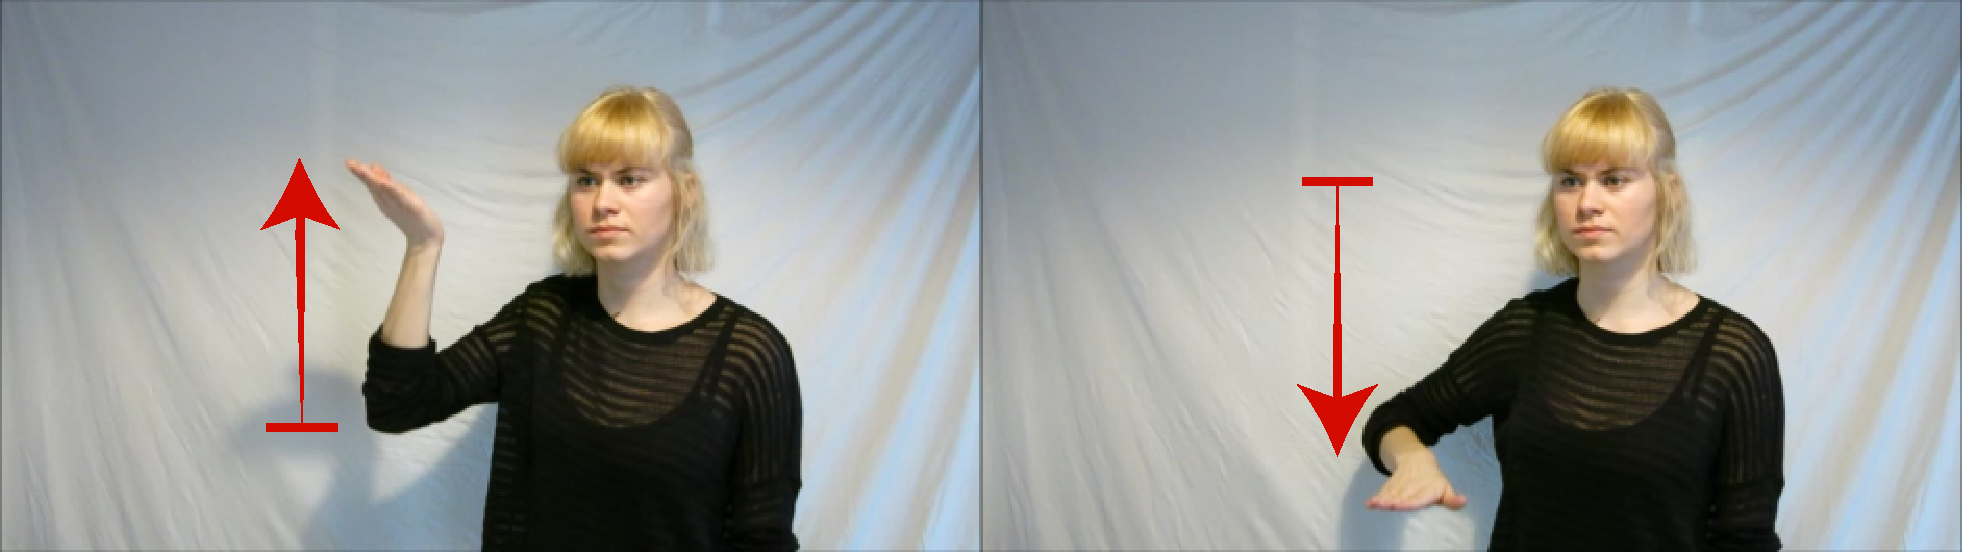
\includegraphics[resolution=300,width=0.9\textwidth]{Test1/Gestik-par/Gestik4_Volumen}
	\caption{Illustration af gestik-par 4; horisontal hånd løftes vertikalt med håndfladen opad for at skrue op og for at skrue ned sænkes hånden vertikalt med håndfladen nedad.}
	\label{fig:GestikPar4Volumen}
\end{figure}
\noindent
%









BEDST 4 
TP2: Nummer 4 er den bedst umiddelbart. Og nummer 5. Og nummer 6 tror jeg.
TP2: Fordi jeg synes de giver mest mening, at det ligesom er op, det betyder op. Man laver en tydelig indikation af hvad der er op og hvad der er ned, hvor jeg synes at den med dreje og sådan noget, der ved man ikke, hvilken vej der er hvad, umiddelbart.
TP2: Fordi jeg synes nummer 4 var mest simpel. Derefter kom nummer 5 som værende mest lignende, synes jeg. Nummer 6 den var sidelæns, så ikke op og ned, så det giver måske ikke lige så meget mening.  


TP12: Jeg kunne meget godt lide de tre, 3, 4 og 5. Fordi der var en op og ned bevægelse. Jeg kunne nok bedst lide nummer 4, som var sådan den her vej (laver gestik 4). Og så 3’eren, fordi det også var bare en hånd. Og 5’eren det er også det der med vandret (hun holder hænderne vandret, men laver en lodret bevægelse). Så 4, 3, 5. 
TP12: Det er det vandrette (hun holder hænderne vandret, men laver bevægelsen lodret) i det, det synes jeg virker naturligt i stedet for at noget cirkel eller den anden vej. 
TP12: Jeg tror det i forhold til hvad jeg selv tænkte var mest naturligt for mig. Og så kunne jeg bedst lide det med en hånd frem for to. 

TP18: 4 er nok den bedste hvis det er bare håndfladen opad (laver gestik 4) og håndfladen nedad (laver gestik 4) så er 4’eren den bedste, og så 9’eren nej 2’eren først og så 9’eren. 
TP18: 4’eren fordi igen det er en simpel bevægelse op ned, der er ikke noget du skal ikke have armen på en eller anden speciel måde du skal bare løfte hånden (laver gestik 4 op) eller træk den nedad (laver gestik 4 ned) altså det giver mening. 2’eren fordi der er et eller andet behageligt over det der med at du drejer lyden op, altså det giver mening også (laver gestik 2).  Det er det du er vant til at gøre at dreje op på et gammeldags anlæg, hvor mange af jer der nu så efterhånden har prøvet det (laver gestik 2). Men den giver mening du drejer lyden op, du skruer lyden op ligesom det hedder (laver gestik 2). Og så den sidste (9) fordi den er simpel, altså igen du kan lave den her siddende du kan gøre sådan her det er det nemmeste tænker jeg (laver gestik 9)
TP18:  Jamen jeg er faktisk også i tvivl om det, fordi jeg syntes 4’eren og 2’eren er begge to stort set ens. Jeg tror bare at det er fordi det giver mening bare at gøre sådan her (laver gestik 4) jeg skal have mere lyd eller jeg skal have mindre lyd (laver gestik 4). Så hvis jeg skulle vælge så vil jeg nok heller gøre den gestus end at jeg skulle den der (laver gestik 2). Det eneste jeg frygter vil være det der med om den kan hvis man gøre sådan her af en eller anden årsag (laver gestik 4) at den så også læser det eller hvis jeg gør sådan her (laver gestik 4 med begge hænder) om den så også læse det som jeg vil vende håndfladen opad. I forhold til hvor man kan sige at det her er en specifik (laver gestik 2) der vil jeg ikke der bør den ikke kunne tage fejl af at jeg nu drejer på lyden. Men hvis man kunne sørge for at den ikke gjorde det ved 4’eren så ville jeg tænke at det er den nemmeste. Simplicitet. 


 


BEDST 5 

BEDST 9 
TP3: Den her den var meget sej, 9’eren. 1’eren skal det ikke være, så giver 2’eren mere mening. Jeg tror 4’eren vil jeg nok sige er den bedste, så 2 og så 9. (efter at prøve det med musik) Jeg tror faktisk det er federe bare at gøre sådan her (Gestik 9), ja, det er meget smartere
TP3: 6 og 7 de er underlige (sagt under spørgsmål 1). Det giver mest mening synes jeg. Det giver mest mening at man løfter et eller andet. Så løfter man et eller andet op og så skubber man det ned. Jeg tænker det giver sådan mest mening at det er lodret, jeg tænker mest med lyd op og ned, sikkert fra computere og sådan noget. Jeg synes også 2’eren giver mening sådan i forhold til at skrue op for en volumen-knap.

TP9: 1’eren som den bedste, og så var det 9’eren, den kunne jeg også godt lide, og 4’eren. Og faktisk også den rækkefølge. (efter at have prøvet det til sidst) Jeg tror faktisk gerne jeg vil skrue trække min 1’er tilbage og så bruge gestik 9 til at skrue op og ned. Fordi da jeg skulle til at skrue op, der kom jeg til at starte med at gøre sådan her (gestik 9), og så kunne jeg godt se det måske var mere naturligt.
TP9: Fordi når man nu står med ungen på den ene arm, så kan man nøjes med bare at bruge en arm til at gøre det ene og det andet. Og den der (gestik 1) virkede forholdsvis overskuelig, og den anden vej virker også forholdsvis nemt. Den her (gestik 2) - stor og klodset. 9’eren er også sådan meget naturligt, kom nu op i gang. 4’eren er ca det samme som 9’eren. 
TP9: Hvad kræver mest bevægelse, for når nu man står på en unge på armen og man så skal lave den her herover (viser gestik med anden hånd), så hvis man laver et eller andet helt vildt, så flyver hun jo med rundt og så taber man hende ud af favnen. Så det er sådan set hvad kræver mindst arbejde af den ene arm og hvad distrahere hende mindst, så hun ikke griber ud efter det og dratter ned på gulvet. 





BEDST 1:
TP8: Jeg tænker i hvert fald gestik 1, det var den jeg sådan bedst kunne lide. Og så tænkte jeg både 3 og 4 virker meget ens, men jeg tænkte sådan 4’eren først og så 3’eren. 
TP8: Først og fremmest, 1’eren det er sådan, det virker sådan meget naturligt, fordi det er det man er sådan vant til med at skrue op. Men i forhold til 2’eren, hvor det er hele hånden der bevæger sig, så er det mere sådan en tydelig bevægelse af at det er det her man gør. Gestik 3 og 4, det er måske sådan lidt af den baggrund jeg har, jeg har en bachelor i musik, det er samme gestik man bruger, når man skal dirigere et kor og få dem til at stige i volumen og falde i volumen. 
TP8: Det var nok sådan mest hvad jeg selv kunne se mig gøre, for at kunne skrue op og ned. 

TP16: Åårh jeg syntes at det nummer 1, nej jeg tror faktisk at jeg vil sige, jo nummer 1, og nummer 4, nej det kan godt være at jeg siger 3 istedet for 4 og så syntes jeg nummer 9 var meget smart (så 1, 3 og 9?) Ja. 
TP16: Altså fordi de giver meget god mening i forhold til at nummer 1 er sådan meget i forhold til at skulle bruge en knap og så grunden til at jeg ikke tog nummer 2 der, for den er jo lidt det samme, det er fordi jeg syntes at det så lidt ukomfortabelt ud og så lagde jeg mærke til at hun (referer til videoen) skruede den forkerte vej i forhold til hvad jeg ville syntes var naturligt (I filmen demonstrer TP hvad det er hun mener der er forkert, TP mener at i videoen bliver det skruet ned ved at dreje hånden med uret og skruet op ved at dreje hånden mod uret, hvilket er omvendt af hvad der faktisk bliver illustreret - der bliver gjort det samme ved 1 og 2 bortset fra antallet af fingre) og det syntes jeg ikke er naturligt for mig. (Hvis du så fik lov til at ændre på den ville det så..(afbrudt)) Ja helt sikkert, det kunne være fint hvis det bare var omvendt, men jeg syntes stadig 1’eren er bedre fordi den var mere, den så mere behagelig ud.   
TP16: Ja, det er rimelig svært for jeg syntes faktisk at de alle sammen var ret fine, men nummer 1 giver sig selv, det er ligesom en knap. Var det så ikke nummer 3 jeg tog? (jo) det er fordi det giver også meget god mening, det er jo bare op ned, ikke (laver gestik 3) og så nummer 9 hvordan var det nu den var (testleder demonstrere), ja det er fordi at det er også sådan lidt smart og en hurtig manøvre man lige hurtig kan smide ud, ikke. 

ANDEN BEDST 1
TP4: 3’eren som nummer 1. Og så nummer 1 og så nummer 2.
TP4: 3’eren fordi den passer godt sammen med det start-stop, så kan man starte den og så køre videre med min hånd, så det passer godt ind der. Og så 1’eren og 2’eren fordi de er meget, det er sådan det man tænker, hvis man vil skrue op og ned for et eller andet, så ligger den meget naturligt. 

TP5: Jeg kan rigtig godt lide den med volume-knappen, men det er også fordi at jeg er vant til volume-knappen, så det ser jeg meget som en selvfølge, at det er det man bruger. Jeg kan også godt lide den her gestik (gestik 6), med at du skruer op på den her måde. Det synes jeg er lidt bedre end opad, det synes jeg fylder mere i rummet, hvis jeg gør sådan her (gestik 5), hvor det her (gestik 6) er mere neutralt, det kan man altid lige hurtigt gøre, uden at skulle til at fylde i rummet. Jeg tror jeg vil gøre det sådan her (kører begge hænder ud til siden), for så skal jeg ikke fokusere på den ene hånd skal holdes stille, så tror jeg det vil være nemmere for mig at gøre det sådan her. Så den vil jeg vælge som nummer 1. Og så bagefter vil jeg nok vælge den med bare fingeren (nummer 1). Den vil også være god synes jeg. Hvis det skal være nummer 3, så skal det være den her, hvor man skruer sådan op (gestik 5) opad. 6, 1 og 5 vil jeg vælge som top 3.
TP5: Fordi jeg synes at gestik 6, der har du mulighed for at bestemme, der kan man ligesom kontrollere det mere - snakker vi 100 kroner eller 1000 kroner - det synes jeg er et meget godt mål. Det er også noget kropssprog man bruger normalt, når man bare snakker. Den her (gestik 1) er meget intuitiv og nem at forstå, og den kan man sådan lave overalt, om det er hernede eller heroppe, den kræver ikke et rum for at man kan lave den. Og 5’eren, jeg synes bare det samme med at du ligesom har kontrol over hvor meget vil du skrue op og ned for noget, det er nemmere at kontrollere med to hænder end det er med en hånd, derfor ville jeg vælge den. Jeg gik fra 2’eren fordi jeg synes den var langsom at bruge. Hvis jeg skal skrue op, så skal jeg gøre sådan her (drejer håndleddet) flere gange, hvor her (gestik 1) kan jeg bare køre 4 gange op. Hvis jeg vil have høj musik, så kan jeg køre hurtigere op. 
TP5: Der har jeg rangeret nummer 6, fordi at som jeg sagde, du kan virkelig godt kontrollere din volumen. Det er nemt med hænder, og du bruger også meget kropssprog, det er noget vi er vant til. Det er måske også farligt, men det er ikke jer der skal forholde jer til det. Så den synes jeg var god og vigtig, god kontrol, og når man snakker om størrelser og mængder, så plejer man også at bruge hænderne for at sige at det er det her vi snakker om, så det synes jeg er en god måde. Og så den anden, nummer 1, den synes jeg er meget intuitiv og nem at forstå. Man kan skrue hurtigt op, man kan skrue hurtigt ned. Jeg ved ikke hvordan det fungerer. Det kan være store cirkler, det kan være små cirker, altså det er jo også godt for folk er forskellige. Folk er forskellige, og hvis du står til en fest, så er det ikke alle der har lyst til at stå sådan her (står med strakte arme ud til siden/over hovedet). hvis det var skrue op, så var der nok ikke så mange der gad at skrue op. Derfor kan jeg også bedre lide den her (gestik 6) end den her (gestik 5), hvor jeg føler man er mere udsat. Men jeg synes stadig den er god, nummer 5, af de andre, der synes jeg det er den bedste af de øvrige, fordi du har noget at måle ud fra. Du har ligesom et referencepunkt, hvor du kan skrue op fra. Hvor de andre der kan du skrue op, og når du så skal til at skrue ned så skal du “fange” det rigtige sted.

TP9: 1’eren som den bedste, og så var det 9’eren, den kunne jeg også godt lide, og 4’eren. Og faktisk også den rækkefølge. (efter at have prøvet det til sidst) Jeg tror faktisk gerne jeg vil skrue trække min 1’er tilbage og så bruge gestik 9 til at skrue op og ned. Fordi da jeg skulle til at skrue op, der kom jeg til at starte med at gøre sådan her (gestik 9), og så kunne jeg godt se det måske var mere naturligt.
TP9: Fordi når man nu står med ungen på den ene arm, så kan man nøjes med bare at bruge en arm til at gøre det ene og det andet. Og den der (gestik 1) virkede forholdsvis overskuelig, og den anden vej virker også forholdsvis nemt. Den her (gestik 2) - stor og klodset. 9’eren er også sådan meget naturligt, kom nu op i gang. 4’eren er ca det samme som 9’eren. 
TP9: Hvad kræver mest bevægelse, for når nu man står på en unge på armen og man så skal lave den her herover (viser gestik med anden hånd), så hvis man laver et eller andet helt vildt, så flyver hun jo med rundt og så taber man hende ud af favnen. Så det er sådan set hvad kræver mindst arbejde af den ene arm og hvad distrahere hende mindst, så hun ikke griber ud efter det og dratter ned på gulvet. 

TREDJE BEDST 1

TP13: Jeg syntes jo at de fleste af dem der tænker man jo sådan det giver mening at det er lyden du. Den tredje bedste vil jeg sige er 1’eren, den der hvor du drejer rundt (laver gestik 1) og den anden bedste det er så 2’eren hvor man sådan kører rundt (laver gestik 2) og så den første, det vil så være 5’eren tror jeg (laver gestik 5) det der med at løfte den op og ned 
TP13: Altså jeg kan bedst lide, jeg kan meget godt lide dem hvor du skruer op og ned (hæver og sænker hånden) og så 5’eren der tænkte jeg at du lige har lidt ekstra med at du skal have begge hænder, men det kan også være en træls ting egentligt at man skal bruge begge hænder (laver gestik 5). Det kan være det er bedre at man kun skal bruge den ene hånd (hvorfor?) hvis man nu laver noget andet og man lige vil skrue op og ned så skal man ikke til at slippe alt man har for at skrue op. (har du lyst til at ændre din top 3?) hvad var forskellen på 3 og 4? (demonstrer) ja så vil jeg nok sige at 3’eren så var den bedste for det er nemt at man bare lige kan gøre det der (laver gestik 3) - (så det skal hedde 3, 2, 1?) ja.  
TP13: Ja, fordi jeg godt kan lide det der, at de kørte, at man skruer op og ned (laver gestik 3) og jeg kunne godt lide at det var lige som en knap (laver gestik 2) man skulle køre rundt med det syntes jeg var lidt sjovt. Og så ja jeg ved ikke helt hvorfor lige præcis den rækkefølge, det føltes rigtigt  




BEDST 2
TP1: Den bedste synes jeg er nummer 2. Den kom jeg i tanke om allerede inden jeg så dem. Så kan jeg også godt lide 6’eren. Den vil jeg rangere som nummer 2. Og så nummer 3 som nummer 3.
TP1: 2’eren, fordi det synes jeg virker mest naturligt, det er ligesom at dreje på en knap, som man gør på gamle stereoanlæg. Så synes jeg det der princip med når man skal vælge noget der er større eller mindre, så ligger det meget naturligt det man gør i 6’eren, derfor har jeg den som 2’eren. Og ja, 3’eren giver også mening i forhold til hvordan man plejer at visualisere lyd på en computer, at det er sådan en bar op og ned, så giver det også god mening at sætte den sådan. Det der med at dreje med 1’eren tror jeg er besværligt i forhold til 2’eren. Jeg tror også det er besværligt den der vej (lavet gestik 5). 4’eren det synes jeg også var underligt at skulle vende hånden. 
TP1: 2’eren synes jeg bare helt klart er det mest naturlige. Det er sådan det man tænker først på, hvis man skal skrue op. Så er det også det der minder mest om de funktioner jeg har oplevet før, hvor man skal dreje på.

TP7:  Jeg tror det er 2 og så 5 og 3. 
TP7: 2’eren fordi at det virker mest naturligt, man er sådan lidt med på at du drejer en knap, man forstår sådan lidt hvad det går ud på. Og så 5’eren fordi at det virker sådan at man har mere kontrol der i forhold til 9’eren, hvor du bare står sådan og vifter opad. Det kunne jo være hvilken som helst volumen du var kommet op på, hvor ved 5’eren kan du sådan skrue helt ned. Og så 3’eren fordi det er sådan lidt en blanding af de to. 

TP14: Altså skal jeg rangere dem alle sammen? (nej kun de tre bedste) jeg tror bedst jeg kunne lide 2’eren, 6’eren og ja 5’eren
TP14: Fordi at jeg tænkte med det samme da jeg så de andre at det er meget naturligt hvad man ellers gør altså i kropssproget, så det måske godt kunne forvirre det, det ved jeg ikke, jeg ved ikke så meget om det, at det vil egentlig være nogle tilpas akavede bevægelser så det ikke vil forstyrre alt muligt andet (laver gestik 2) og ikke minde om naturlige gestikker, som du kan se så er jeg ret meget gestikulerende i den måde jeg taler naturligt (laver bevægelser) så tænker jeg at det ville kunne forstyrre det og 2’eren tænker jeg at er en akavet bevægelse, som jeg nok ikke naturligt vil gøre (laver gestik 2). Det er min umiddelbare tanke hvertfald.  
TP14: Igen det der med at jeg tænker 2’eren er den mest akavede egentlig (laver gestik 2) eller den mest unaturlige bevægelse af de andre så den syntes jeg virkede bedst og 6’eren efter samme princip at det er det jeg tænker

TP17: Det ved jeg ikke, den bedste er 2’eren og den anden bedste er den sidste (9eren) og 7’eren giver meget god mening hvis man rører ved det.  (Hvis du ikke rører ved det) så er det 3 (så 2, 9 og 3?) ja.
TP17: 2’eren giver bare god mening for det er ligesom man har gjort i gamle dage (laver gestik 2) og den sidste syntes jeg bare er meget smart, fordi man sådan kan (laver gestik 9), det andet skal man til at huske at bruge begge hænder, den anden der er sådan lidt mere logisk, syntes jeg og den sidste ja det er også bare sådan at man bruger hænderne, det er jo faktisk lidt på samme måde som 9eren det er bare at køre med hånden i stedet for (laver gestik 3). Jeg syntes 2’eren den var ret smart
TP17: Ja, 2’eren det er 2’eren fordi jeg er vant til at køre bil det er sådan jeg tænder og slukker for den og den anden er bare en meget logisk (laver gestik 9) syntes jeg altså sådan det er sådan lidt, jeg ville ikke tænke over det at jeg skulle skrue op og ned, det skulle bare være sådan helt naturligt.

ANDEN BEDST 2: 
TP13: Jeg syntes jo at de fleste af dem der tænker man jo sådan det giver mening at det er lyden du. Den tredje bedste vil jeg sige er 1’eren, den der hvor du drejer rundt (laver gestik 1) og den anden bedste det er så 2’eren hvor man sådan kører rundt (laver gestik 2) og så den første, det vil så være 5’eren tror jeg (laver gestik 5) det der med at løfte den op og ned 
TP13: Altså jeg kan bedst lide, jeg kan meget godt lide dem hvor du skruer op og ned (hæver og sænker hånden) og så 5’eren der tænkte jeg at du lige har lidt ekstra med at du skal have begge hænder, men det kan også være en træls ting egentligt at man skal bruge begge hænder (laver gestik 5). Det kan være det er bedre at man kun skal bruge den ene hånd (hvorfor?) hvis man nu laver noget andet og man lige vil skrue op og ned så skal man ikke til at slippe alt man har for at skrue op. (har du lyst til at ændre din top 3?) hvad var forskellen på 3 og 4? (demonstrer) ja så vil jeg nok sige at 3’eren så var den bedste for det er nemt at man bare lige kan gøre det der (laver gestik 3) - (så det skal hedde 3, 2, 1?) ja.  
TP13: Ja, fordi jeg godt kan lide det der, at de kørte, at man skruer op og ned (laver gestik 3) og jeg kunne godt lide at det var lige som en knap (laver gestik 2) man skulle køre rundt med det syntes jeg var lidt sjovt. Og så ja jeg ved ikke helt hvorfor lige præcis den rækkefølge, det føltes rigtigt  

TP18: 4 er nok den bedste hvis det er bare håndfladen opad (laver gestik 4) og håndfladen nedad (laver gestik 4) så er 4’eren den bedste, og så 9’eren nej 2’eren først og så 9’eren. 
TP18: 4’eren fordi igen det er en simpel bevægelse op ned, der er ikke noget du skal ikke have armen på en eller anden speciel måde du skal bare løfte hånden (laver gestik 4 op) eller træk den nedad (laver gestik 4 ned) altså det giver mening. 2’eren fordi der er et eller andet behageligt over det der med at du drejer lyden op, altså det giver mening også (laver gestik 2).  Det er det du er vant til at gøre at dreje op på et gammeldags anlæg, hvor mange af jer der nu så efterhånden har prøvet det (laver gestik 2). Men den giver mening du drejer lyden op, du skruer lyden op ligesom det hedder (laver gestik 2). Og så den sidste (9) fordi den er simpel, altså igen du kan lave den her siddende du kan gøre sådan her det er det nemmeste tænker jeg (laver gestik 9)
TP18:  Jamen jeg er faktisk også i tvivl om det, fordi jeg syntes 4’eren og 2’eren er begge to stort set ens. Jeg tror bare at det er fordi det giver mening bare at gøre sådan her (laver gestik 4) jeg skal have mere lyd eller jeg skal have mindre lyd (laver gestik 4). Så hvis jeg skulle vælge så vil jeg nok heller gøre den gestus end at jeg skulle den der (laver gestik 2). Det eneste jeg frygter vil være det der med om den kan hvis man gøre sådan her af en eller anden årsag (laver gestik 4) at den så også læser det eller hvis jeg gør sådan her (laver gestik 4 med begge hænder) om den så også læse det som jeg vil vende håndfladen opad. I forhold til hvor man kan sige at det her er en specifik (laver gestik 2) der vil jeg ikke der bør den ikke kunne tage fejl af at jeg nu drejer på lyden. Men hvis man kunne sørge for at den ikke gjorde det ved 4’eren så ville jeg tænke at det er den nemmeste. Simplicitet. 

TREDJE BEDST 2: 
TP3: Den her den var meget sej, 9’eren. 1’eren skal det ikke være, så giver 2’eren mere mening. Jeg tror 4’eren vil jeg nok sige er den bedste, så 2 og så 9. (efter at prøve det med musik) Jeg tror faktisk det er federe bare at gøre sådan her (Gestik 9), ja, det er meget smartere
TP3: 6 og 7 de er underlige (sagt under spørgsmål 1). Det giver mest mening synes jeg. Det giver mest mening at man løfter et eller andet. Så løfter man et eller andet op og så skubber man det ned. Jeg tænker det giver sådan mest mening at det er lodret, jeg tænker mest med lyd op og ned, sikkert fra computere og sådan noget. Jeg synes også 2’eren giver mening sådan i forhold til at skrue op for en volumen-knap.

TP4: 3’eren som nummer 1. Og så nummer 1 og så nummer 2.
TP4: 3’eren fordi den passer godt sammen med det start-stop, så kan man starte den og så køre videre med min hånd, så det passer godt ind der. Og så 1’eren og 2’eren fordi de er meget, det er sådan det man tænker, hvis man vil skrue op og ned for et eller andet, så ligger den meget naturligt. 

TP10: Den bedste det synes jeg var 3’eren. Og så var det nok 5’eren og 2’eren.
TP10: Jamen fordi jeg synes de er sådan meget intuitive måde at gøre det på, det er meget nemt at huske. Når det handler om at skrue op og ned for lyden, så er det ligesom en bevægelse der passer meget godt til det den skal gøre. 
TP10: Hvorfor det lige var i den rækkefølge, jeg kan bedre lide de her køren en hånd op og ned end den hvor du skal dreje, så de kom før den. Og 3’eren øverst bare fordi man kan gøre det med en hånd i forhold til 5’eren.



BEDST 3
TP4: 3’eren som nummer 1. Og så nummer 1 og så nummer 2.
TP4: 3’eren fordi den passer godt sammen med det start-stop, så kan man starte den og så køre videre med min hånd, så det passer godt ind der. Og så 1’eren og 2’eren fordi de er meget, det er sådan det man tænker, hvis man vil skrue op og ned for et eller andet, så ligger den meget naturligt. 

TP6: 3, tror jeg, som den bedste, bare op og ned igen. 4’eren nogenlunde det samme bare med omvendt hånd. Så er det enten 8 eller 9 som er 3’eren tænker jeg. Nok 8 tror jeg, så bare pege op og så ned. 
TP6: De virker nemmest at arbejde med. Køre rundt (gestik 1) kunne jeg forestille mig det er også en måde at gøre det på, men jeg vil nok hellere mere bare løfte hånden. De andre der de er også fine, men ved den her (gestik 5), der ville jeg bare kunne se et problem i at man starter på niveauet musikken allerede kører på og så køre op og så køre ned, og så når du ned på det samme niveau som du havde før. Så hvis nu det var at du gerne ville skrue ned, så kunne jeg forestille mig du muligvis skulle gøre sådan (kører hånden ned under referencehånden). Det virker bare nemmere at kunne køre op og ned hvor du helt præcis vil have den. Muligvis skal man have en mute funktion. Jeg muter kun hvis det ikke er mit musik, hvis der fx kører noget youtube og der kommer nogle reklamer, så er det jo smart at mute lyden der og så, ja, der ville man jo have en funktion, men ellers så nej, jeg muter jo aldrig min musik. 
TP6: Jamen det tror jeg er det der med at det er mere naturligt. Det er en lille smule vigtigere end den der funktionalitet, men det ligger meget tæt. Det er sådan måske nærmest en delt 1. plads. og så 3’eren.


TP10: Den bedste det synes jeg var 3’eren. Og så var det nok 5’eren og 2’eren.
TP10: Jamen fordi jeg synes de er sådan meget intuitive måde at gøre det på, det er meget nemt at huske. Når det handler om at skrue op og ned for lyden, så er det ligesom en bevægelse der passer meget godt til det den skal gøre. 
TP10: Hvorfor det lige var i den rækkefølge, jeg kan bedre lide de her køren en hånd op og ned end den hvor du skal dreje, så de kom før den. Og 3’eren øverst bare fordi man kan gøre det med en hånd i forhold til 5’eren.


TP11: Jeg tror den jeg bedst kan lide det er gestik nummer 3. Og så må det nok være 4, 8.
TP11: Jeg synes det er måske de mest intuitive bevægelser. Hvis du vil have noget op, så er det en opadgående bevægelse. Hvor jeg synes det vil være lidt irriterende at skulle sidde sådan (drejer med hånden som gestik 2), så vil det være lidt mere logisk på en eller anden måde (laver gestik 3).
TP11: Fordi 4’eren der synes jeg det er lidt træls den skelner mellem selve håndbevægelsen, hvor du burde måske bare kunne løfte hånden, hvis det skal være. Og så 8’eren, det er egentlig også smart nok, men jeg tror bare jeg er mere fan af det der intuitive med at du kan køre hånden op og ned. 


TP13: Jeg syntes jo at de fleste af dem der tænker man jo sådan det giver mening at det er lyden du. Den tredje bedste vil jeg sige er 1’eren, den der hvor du drejer rundt (laver gestik 1) og den anden bedste det er så 2’eren hvor man sådan kører rundt (laver gestik 2) og så den første, det vil så være 5’eren tror jeg (laver gestik 5) det der med at løfte den op og ned 
TP13: Altså jeg kan bedst lide, jeg kan meget godt lide dem hvor du skruer op og ned (hæver og sænker hånden) og så 5’eren der tænkte jeg at du lige har lidt ekstra med at du skal have begge hænder, men det kan også være en træls ting egentligt at man skal bruge begge hænder (laver gestik 5). Det kan være det er bedre at man kun skal bruge den ene hånd (hvorfor?) hvis man nu laver noget andet og man lige vil skrue op og ned så skal man ikke til at slippe alt man har for at skrue op. (har du lyst til at ændre din top 3?) hvad var forskellen på 3 og 4? (demonstrer) ja så vil jeg nok sige at 3’eren så var den bedste for det er nemt at man bare lige kan gøre det der (laver gestik 3) - (så det skal hedde 3, 2, 1?) ja.  
TP13: Ja, fordi jeg godt kan lide det der, at de kørte, at man skruer op og ned (laver gestik 3) og jeg kunne godt lide at det var lige som en knap (laver gestik 2) man skulle køre rundt med det syntes jeg var lidt sjovt. Og så ja jeg ved ikke helt hvorfor lige præcis den rækkefølge, det føltes rigtigt  


TP15: Der var det nummer 3, som den bedste og så nummer 4 som nummer to og så nummer 9 
TP15: Fordi at jeg syntes det var meget logisk at den måde - ja den første der, da 3’eren kom så  tænkte jeg at det var også sådan jeg syntes at det var mest logisk (laver bevægelsen), men så nummer 4 så blev det lige lidt mere kompliceret med at man skulle vende hånden, men så tænkte jeg ved nummer 9 eller 8 at det godt kunne være at de ikke kunne registreres ordentligt så  - (demonstrere) ja jeg syntes at det er meget smart, men det kunne være at hvis det ikke var det rigtige apparat at den ikke lige ville kunne registrere det ordentligt 
TP15: Fordi jeg syntes at det var dem der var mest simple, og så syntes jeg f.eks. at nummer 5 og 6, 5’eren den var også meget simpel men så skal til at bruge begge hænder og 6’eren den gav lidt mindre mening at gøre det på den led. 

ANDEN BEDST 3
TP12: Jeg kunne meget godt lide de tre, 3, 4 og 5. Fordi der var en op og ned bevægelse. Jeg kunne nok bedst lide nummer 4, som var sådan den her vej (laver gestik 4). Og så 3’eren, fordi det også var bare en hånd. Og 5’eren det er også det der med vandret (hun holder hænderne vandret, men laver en lodret bevægelse). Så 4, 3, 5. 
TP12: Det er det vandrette (hun holder hænderne vandret, men laver bevægelsen lodret) i det, det synes jeg virker naturligt i stedet for at noget cirkel eller den anden vej. 
TP12: Jeg tror det i forhold til hvad jeg selv tænkte var mest naturligt for mig. Og så kunne jeg bedst lide det med en hånd frem for to. 

TP16: Åårh jeg syntes at det nummer 1, nej jeg tror faktisk at jeg vil sige, jo nummer 1, og nummer 4, nej det kan godt være at jeg siger 3 istedet for 4 og så syntes jeg nummer 9 var meget smart (så 1, 3 og 9?) Ja. 
TP16: Altså fordi de giver meget god mening i forhold til at nummer 1 er sådan meget i forhold til at skulle bruge en knap og så grunden til at jeg ikke tog nummer 2 der, for den er jo lidt det samme, det er fordi jeg syntes at det så lidt ukomfortabelt ud og så lagde jeg mærke til at hun (referer til videoen) skruede den forkerte vej i forhold til hvad jeg ville syntes var naturligt (I filmen demonstrer TP hvad det er hun mener der er forkert, TP mener at i videoen bliver det skruet ned ved at dreje hånden med uret og skruet op ved at dreje hånden mod uret, hvilket er omvendt af hvad der faktisk bliver illustreret - der bliver gjort det samme ved 1 og 2 bortset fra antallet af fingre) og det syntes jeg ikke er naturligt for mig. (Hvis du så fik lov til at ændre på den ville det så..(afbrudt)) Ja helt sikkert, det kunne være fint hvis det bare var omvendt, men jeg syntes stadig 1’eren er bedre fordi den var mere, den så mere behagelig ud.   
TP16: Ja, det er rimelig svært for jeg syntes faktisk at de alle sammen var ret fine, men nummer 1 giver sig selv, det er ligesom en knap. Var det så ikke nummer 3 jeg tog? (jo) det er fordi det giver også meget god mening, det er jo bare op ned, ikke (laver gestik 3) og så nummer 9 hvordan var det nu den var (testleder demonstrere), ja det er fordi at det er også sådan lidt smart og en hurtig manøvre man lige hurtig kan smide ud, ikke.



TREDJE BEDST 3
TP1: Den bedste synes jeg er nummer 2. Den kom jeg i tanke om allerede inden jeg så dem. Så kan jeg også godt lide 6’eren. Den vil jeg rangere som nummer 2. Og så nummer 3 som nummer 3.
TP1: 2’eren, fordi det synes jeg virker mest naturligt, det er ligesom at dreje på en knap, som man gør på gamle stereoanlæg. Så synes jeg det der princip med når man skal vælge noget der er større eller mindre, så ligger det meget naturligt det man gør i 6’eren, derfor har jeg den som 2’eren. Og ja, 3’eren giver også mening i forhold til hvordan man plejer at visualisere lyd på en computer, at det er sådan en bar op og ned, så giver det også god mening at sætte den sådan. Det der med at dreje med 1’eren tror jeg er besværligt i forhold til 2’eren. Jeg tror også det er besværligt den der vej (lavet gestik 5). 4’eren det synes jeg også var underligt at skulle vende hånden. 
TP1: 2’eren synes jeg bare helt klart er det mest naturlige. Det er sådan det man tænker først på, hvis man skal skrue op. Så er det også det der minder mest om de funktioner jeg har oplevet før, hvor man skal dreje på.

TP7:  Jeg tror det er 2 og så 5 og 3. 
TP7: 2’eren fordi at det virker mest naturligt, man er sådan lidt med på at du drejer en knap, man forstår sådan lidt hvad det går ud på. Og så 5’eren fordi at det virker sådan at man har mere kontrol der i forhold til 9’eren, hvor du bare står sådan og vifter opad. Det kunne jo være hvilken som helst volumen du var kommet op på, hvor ved 5’eren kan du sådan skrue helt ned. Og så 3’eren fordi det er sådan lidt en blanding af de to. 

TP8: Jeg tænker i hvert fald gestik 1, det var den jeg sådan bedst kunne lide. Og så tænkte jeg både 3 og 4 virker meget ens, men jeg tænkte sådan 4’eren først og så 3’eren. 
TP8: Først og fremmest, 1’eren det er sådan, det virker sådan meget naturligt, fordi det er det man er sådan vant til med at skrue op. Men i forhold til 2’eren, hvor det er hele hånden der bevæger sig, så er det mere sådan en tydelig bevægelse af at det er det her man gør. Gestik 3 og 4, det er måske sådan lidt af den baggrund jeg har, jeg har en bachelor i musik, det er samme gestik man bruger, når man skal dirigere et kor og få dem til at stige i volumen og falde i volumen. 
TP8: Det var nok sådan mest hvad jeg selv kunne se mig gøre, for at kunne skrue op og ned.

TP17: Det ved jeg ikke, den bedste er 2’eren og den anden bedste er den sidste (9eren) og 7’eren giver meget god mening hvis man rører ved det.  (Hvis du ikke rører ved det) så er det 3 (så 2, 9 og 3?) ja.
TP17: 2’eren giver bare god mening for det er ligesom man har gjort i gamle dage (laver gestik 2) og den sidste syntes jeg bare er meget smart, fordi man sådan kan (laver gestik 9), det andet skal man til at huske at bruge begge hænder, den anden der er sådan lidt mere logisk, syntes jeg og den sidste ja det er også bare sådan at man bruger hænderne, det er jo faktisk lidt på samme måde som 9eren det er bare at køre med hånden i stedet for (laver gestik 3). Jeg syntes 2’eren den var ret smart
TP17: Ja, 2’eren det er 2’eren fordi jeg er vant til at køre bil det er sådan jeg tænder og slukker for den og den anden er bare en meget logisk (laver gestik 9) syntes jeg altså sådan det er sådan lidt, jeg ville ikke tænke over det at jeg skulle skrue op og ned, det skulle bare være sådan helt naturligt.

















